\documentclass{report}

\newenvironment{eq}[0]{
	\begin{equation}
	\begin{aligned}
}{
	\end{aligned}
	\end{equation}
}
\newenvironment{eq*}[0]{
	\begin{equation*}
	\begin{aligned}
}{
	\end{aligned}
	\end{equation*}
}
\usepackage{mathtools}
\usepackage{amssymb}
\usepackage{graphicx}
\newcommand*\rfrac[2]{{}^{#1}\!/_{#2}}

\author{Kaare Hoff Skovgaard (20092804)}
\title{Handin 2 - Optimization F14}


\begin{document}
	\maketitle

	By simply reading and understanding the problem given, quickly it is seen that the linear program is:

	Maximize:
	\begin{eq*}
		300 x_1 + 100 x_2
	\end{eq*}
	Subject to:
	\begin{eq*}
		6 x_1 + 3 x_2 &\leq 40 \\
		3 x_1 - x_2 &\leq 0 \\
		x_1 + \rfrac{1}{4} x_2 &\leq 4
	\end{eq*}

	Which can then be seen graphically below:

	\begin{figure}[ht!]
		\centering
		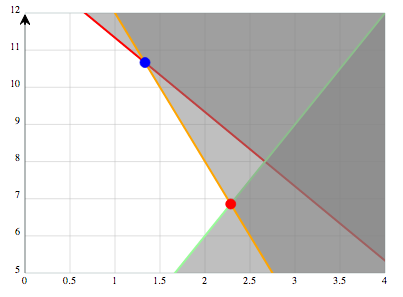
\includegraphics[width=90mm]{afl2_graph.png}
		\caption{A simple graph showing the solution. The white area is the feasible solution area}
		\label{fig:graph}
	\end{figure}

	By solving the equations we can find the points of intersections, the intersection points that are marked in Figure \ref{fig:graph} are:

	\begin{enumerate}
		\item[Blue dot] $x_1 = \rfrac{4}{3}, x_2 = \rfrac{32}{3}$
		\item[Red dot] $x_1 = \rfrac{16}{7}, x_2 = \rfrac{48}{7}$
	\end{enumerate}

	Yielding the maximum profit is the blue dot, at $1466 + 2/3$ DKK per week.
\end{document}
